\subsection{Солнечное излучение. Солнечная постоянная. Распределение энергии по спектру.}
См. вопрос \ref{q5-1}.

До поверхности Земли доходит (см. рис. \ref{fig:J_sun}):
\begin{itemize}
\item Ультрафиолетовое излучение (0.2 -- 0.4 мкм) -- 10 \% интенсивности. Поглощается озоном.
\item Видимое излучение (0.4 -- 0.75 мкм) -- 45 \% интенсивности. Рассеивается молекулами газов и находящимися в воздухе частицами пыли и аэрозоля.
\item Инфракрасное (тепловое) излучение (0.75 -- 1000 мкм) -- 45 \% интенсивности. Поглощается водяным паром.
\end{itemize}

\begin{figure}[!ht]
\centering
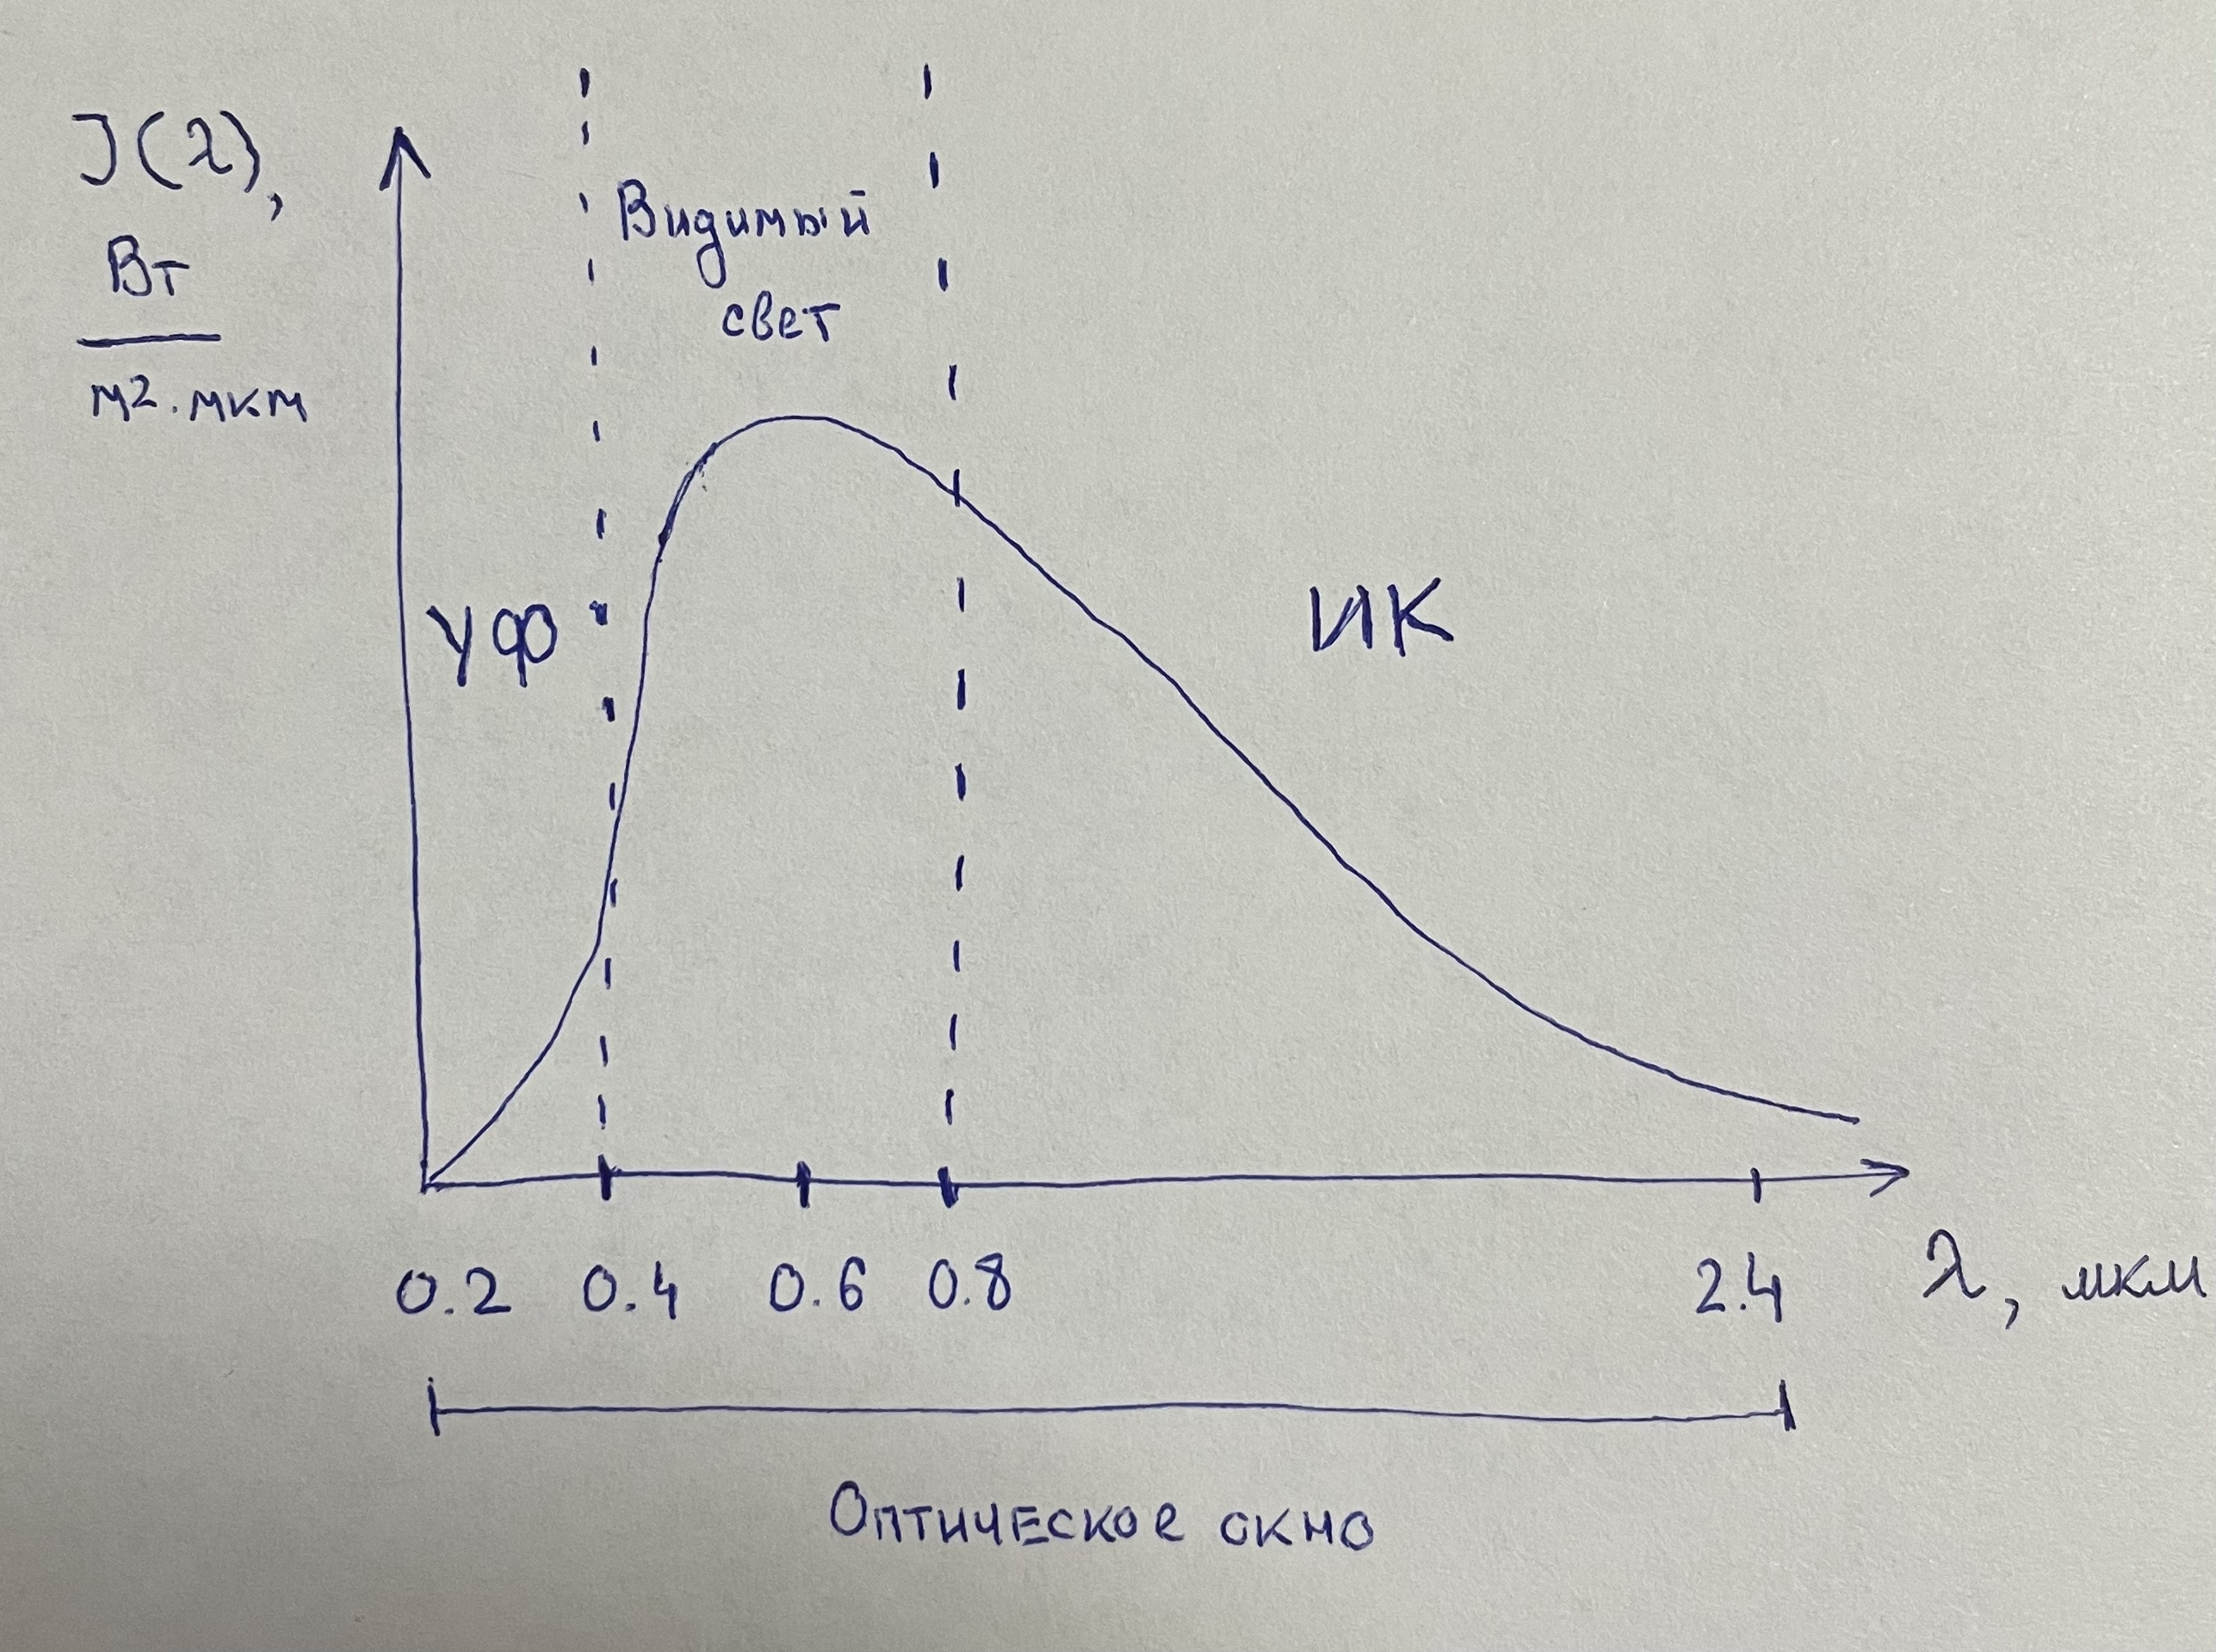
\includegraphics[width=0.5\textwidth]{images/J_sun.png}
\caption{Спектральная плотность потока солнечной радиации. Оптическое окно -- диапазон длин волн, на который приходится основная часть (свыше 95 \%) энергии Солнца.}\label{fig:J_sun}
\end{figure}
